\documentclass[beamer,9pt,aspectratio=169]{beamer}
\usetheme{Madrid}
\usecolortheme{orchid}
\usepackage[utf8]{inputenc}
\usepackage[portuguese]{babel}
\usepackage[T1]{fontenc}
%\usepackage[a4paper]{geometry}
\usepackage{icomma, amsmath, tikz, physics}


\usetikzlibrary{decorations.pathreplacing,
                decorations.markings,
                decorations.text,
                arrows,
                shapes.geometric,
                shapes.misc,
                intersections}

%\setbeamersize{text margin left=0.1mm, text margin right=.5mm}
\setlength{\leftmargini}{1.0em}
%\setlength{\leftmarginii}{0.90em}
%\setlength{\leftmarginiii}{1.25em}
\setbeamertemplate{itemize item}{}

%remove Madrid footer, navigation buttons, add gray frame numbers
\setbeamercolor{page number in head/foot}{fg=gray}
\setbeamertemplate{footline}[frame number]{}
\setbeamertemplate{navigation symbols}{}
\beamerdefaultoverlayspecification{<+->}

%Thinner frametitle
\makeatletter
\setbeamertemplate{frametitle}{%
  \nointerlineskip
  \begin{beamercolorbox}[ht=1.0em,dp=0.5ex,wd=\paperwidth,leftskip=.1cm,rightskip=0cm]{frametitle}%
    \usebeamerfont{frametitle}\usebeamercolor[fg]{framesubtitle}\insertframetitle
  \end{beamercolorbox}
  \ifx\insertframesubtitle\@empty%
  \else
  \nointerlineskip%
  \begin{beamercolorbox}[sep=.3ex,wd=\paperwidth,leftskip=.5cm,rightskip=0cm]{frametitle}%
  \usebeamerfont{framesubtitle}\usebeamercolor[fg]{framesubtitle}\insertframesubtitle%
  \end{beamercolorbox}
  \fi
}

% Plain enumerate labels
\setbeamertemplate{enumerate items}[default]

\setlength{\parindent}{0mm}
\newcommand*\cancel[2][thin]{%
  \tikz[baseline]
  \node [strike out,draw,anchor=text,inner sep=0pt,text=black,#1]{#2};
}

\begin{document}
%-------------------------------------------------------------------------------
\begin{frame}{Esqueci-me de referir isto na segunda feira!}
\begin{itemize}
  \item Observações de Neptuno por Galileu: 1612
    \vspace{2em}
  \item Descoberta de Urano: 1781 (Hershell)
    \vspace{2em}
  \item Descoberta de Neptuno: 1846 (Galle)
    \vspace{8em}
  \item
    (Todos têm acesso ao moodle da formação?)
\end{itemize}
\end{frame}
%-------------------------------------------------------------------------------
\begin{frame}{Movimento do Sol e planetas relativamente às estrelas fixas}
  \begin{enumerate}
    \setlength{\itemsep}{0.9em}
    \item ``Apague'' a representação da atmosfera e do chão no stellarium.
    \item Ative a observação com uma montagem equatorial.
    \item Encontre o Sol (pesquise com CRTL-F).
    \item Acelere a marcha do tempo no stellarium.
    \item Note como o Sol se move de oeste para leste (no sentido oposto ao
      movimento aparente) relativamente ao fundo das estrelas fixas.
    \item Note como todos os planetas seguem aproximadamente a trajetória do Sol,
      uns mais rapidamente que outros.
    \item Repare que alguns planetas sofrem, mais ou menos frequentemente,
      inversões no sentido do seu movimento (ainda relativamente ao fundo das
      estrelas fixas). É o chamado \emph{movimento retrógrado,} na verdade
      apenas uma manifestação do movimento relativamente à Terra.\\
      {\small\textsf{%
      Em que planetas ocorre mais frequentemente? Quanto tempo duram as fases de
      movimento retrógrado? Essa duração é a mesma para todos?
      }}
    \item
      E cometas?\\ Localize o cometa C/2023 A3 (Tsuchinshan-ATLAS), que será
      visível no hemisfério norte no início de Outubro. Siga o mesmo
      procedimento para observar o seu movimento. Mantém-se também sempre
      próximo da eclítica?
  \end{enumerate}
\end{frame}
%-------------------------------------------------------------------------------
\begin{frame}[label=eratostenes]{Determinação do raio da Terra
  (Eratóstenes, 200\,aC)}
  \begin{minipage}[t]{0.6\linewidth}
    \begin{enumerate}
      \setlength{\itemsep}{1em}
      \item ``Apague'' a atmosfera 
      \item
        Determine um instante em que uma estrela do catálogo se encontre no
        zénite (vertical) do ponto de observação e pare o avanço do tempo nesse
        instante.
      \item
        Mude a localização do observatório virtual para outro ponto na
        superfície da Terra e determine a altitude angular da mesma estrela na
        nova localização. 
      \item
        Determine a amplitude do ângulo entre entre as duas direções de
        observação ($\theta$).
      \item
        Usando o googleearth (por exemplo) determine a distância entre as duas
        localizações ($s$).
    \end{enumerate}

    \vspace{2em}
    \uncover<+->{%
      \begin{equation*}
        R_T=s/\theta
      \end{equation*}
    }
  \end{minipage}\hfill
  \raisebox{-\height}{%
    \includegraphics[width=0.3\linewidth]{figs/f1.png}
  }
\end{frame}
%-------------------------------------------------------------------------------
\begin{frame}{$R_L/R_T$ (Hiparco, 150\,aC) --- 1. Cálculo grosseiro}
  \begin{minipage}[t]{0.5\linewidth}
  \begin{enumerate} 
    \item Procure na internet uma foto da sombra da Terra projetada na Lua
      durante um eclipse lunar parcial. Escolha uma (ou mais) com essa sombra
      bem delimitada
    \item
      Importe a imagem para o geogebra
    \item 
      Ajuste uma circunferência ao disco lunar e outra ao arco da sombra da
      Terra projetada na Lua. O geogebra deve indicar os valores dos quadrados
      dos raios ($r^*_L$ e $r^*_s$) destas circunferências (em unidades arbitrárias)
    \item
      Primeira estimativa: supondo o Sol muito longe, a sombra da Terra é
      cilíndrica; então:
      \begin{equation*}
          \frac{R_T}{R_L}=\frac{r^*_s}{r^*_L}
      \end{equation*}
  \end{enumerate}
  \end{minipage}\hfill
  \raisebox{-\height}{%
    \includegraphics[width=0.45\linewidth]{figs/f3.png}
  }
\end{frame}

%-------------------------------------------------------------------------------
\begin{frame}[label=rtrl]{$R_L/R_T$ (Hiparco, 150\,aC)
  --- 2. Agora mais a sério}
  \includegraphics{figs/f2.png}
  \pause
  \begin{itemize} 
    \item 
      \begin{equation*}
        \left.
          \begin{aligned}
            \triangle FTP:\ &\varepsilon=\alpha +\varphi \\
            \triangle FTD:\ &\beta=\varphi +\delta 
          \end{aligned}
        \right\}
        \implies \varepsilon=\alpha+\beta-\delta
      \end{equation*}
    \item
      $\alpha$ é o raio angular da sombra da Terra projetada na Lua:
      $\alpha=\eta r^*_s/L$, onde $\eta$ é um fator de escala.
    \item 
      $\beta$ é o raio angular do Sol visto da Terra. É aproximadamente
      igual ao raio angular da Lua. Então $\beta = \eta r^*_L/L$
    \item 
      $\varepsilon$ é o raio angular da Terra vista da Lua: $\varepsilon=R_T/L$
    \item 
      $\delta$ é o raio angular da Terra vista do Sol: $\delta\simeq0$
    \item 
      \begin{equation*}
        R_T=\eta (r^*_s+r^*_L)\implies \frac{R_T}{R_L}=1+\frac{r^*_s}{r^*_L}
      \end{equation*}
  \end{itemize}
\end{frame}
%-------------------------------------------------------------------------------
\begin{frame}{$L/S$ (Hiparco, 150\,aC, mas melhor ainda!)}
  \begin{minipage}[t]{0.4\linewidth}
  \begin{center}
    A Lua em quarto crescente
    
    \vspace{2em}
    \includegraphics[width=0.9\linewidth]{figs/f4.png}
  \end{center}
  \pause
  \vspace{3em}
  \begin{equation*}
        \frac{L}{S}=\cos\theta
  \end{equation*}
  \end{minipage}
  \hfill
  \begin{minipage}[t]{0.4\linewidth}
    \pause
    \begin{enumerate}
      \setlength{\itemsep}{2em}
      \item No stellarium, determine um instante de Lua em quadratura (crescente
        ou decrescente, tanto faz).
      \item Pare o andamento do tempo.
      \item Com a ferramente de medição de ângulos determine $\theta$.
    \end{enumerate}
  \end{minipage}
\end{frame}
%-------------------------------------------------------------------------------
\begin{frame}{Novas descobertas}
  \begin{enumerate}
      \setlength{\itemsep}{3em}
    \item
      Agora que conhecemos o raio da Terra (ver o slide \ref{eratostenes})
      e a razão $R_T/R_L$ (slide \ref{rtrl}), podemos determinar o raio da Lua.
    \item Conhecido o raio da Lua, podemos determinar a sua distância a partir
      do seu tamanho angular.
    \item Conhecida a distância à Lua, podemos calcular a distância ao Sol, com o
      cálculo no slide anterior.
  \end{enumerate}
\end{frame}
%-------------------------------------------------------------------------------
\begin{frame}{As fases de Vénus e o modelo heliocêntrico}
  \begin{enumerate}
      \setlength{\itemsep}{2em}
  \item
    Desative a representação da Terra e da atmosfera e pare a marcha do tempo;
  \item
    Localize Vénus (usando o comando de busca, CTRL-F) e centre-o no centro da
    imagem (se Vénus está selecionado, basta pressionar a barra de espaço);
  \item
    Aumente a imagem (zoom in, usando a roda do rato) até o disco de Vénus ter
    uma dimensão apreciável;
  \item
    Ative a janela de Data e Hora e avance o tempo mês a mês;
  \item
    Note como o tamanho do disco de Vénus varia de mês para mês, e correlacione
    essas variações com as fases de iluminação. Quando o disco de Vénus está
    completamente iluminado (Vénus ``cheio''), o seu tamanho é máximo, ou
    mínimo? E quando está completamente escurecido (Vénus ``novo'')? Como
    podemos interpretar estas observações em termos dos modelos geocêntrico e
    heliocêntrico?
\end{enumerate}
\end{frame}
%-------------------------------------------------------------------------------
\begin{frame}{O céu noturno --- Algumas pistas}
  \begin{itemize}
    \item Ursa maior e ursa menor
    \item Orion, Pleiades, Sirius
    \item Cassiopeia e Andrómeda
    \item O triângulo de Verão
    \item Escropião, sagitário e o centro da nossa galáxia
    \item A via látea
  \end{itemize}
\end{frame}
%-------------------------------------------------------------------------------
\begin{frame}{Telescópios}
  \begin{minipage}[t]{0.6\linewidth}
  \vspace{5em}
  \begin{enumerate}[<.->]
    \setlength{\itemsep}{4em}
    \item Como ver objetos com um tamanho aparente demasiado pequeno?
    \item Como ver objetos com luminosidade demasiado ténue?
  \end{enumerate}
  \end{minipage}\hfill
  \raisebox{-\height}{%
    \includegraphics[width=0.39\linewidth]{figs/f6.jpg}
  }
\end{frame}
%-------------------------------------------------------------------------------
\begin{frame}{Telescópios --- Lentes e espelhos}
  \begin{itemize}
    \item
      Lentes convexas e espelhos côncavos fazem, respetivamente por refração e
      reflexão, convergir raios paralelos de luz neles incidentes em direções
      que convergem num mesmo ponto.
    \item Os objetos astronómicos estão muito longe, cada ponto do objeto é
      fonte de raios de luz que chegam à Terra paralelos. Assim, se incidirem numa
      lente ou num espelho convergentes, serão refratados ou refletidos
      convergindo para um ponto, o \emph{ponto imagem} do ponto fonte de luz
      \begin{center}
        \includegraphics[width=0.5\linewidth]{figs/f5.png}
      \end{center}
    \item Se colocarmos um sensor fotográfico (CCD) no plano focal, pode
      registar-se a imagem refratada ou refletida.
    \item
      As imagens de dois objetos celestes pontuais separados por uma distância
      angular $\delta$ ficam separadas no plano focal por uma distância
      \begin{equation*}
        d=f\tan\delta\simeq d\delta.
      \end{equation*}
    \item Ou seja, quanto maior a distância focal da lente ou do espelho,
      melhor.
      \vspace{0.85em}
    \item
      {\color{gray}
        Em rigor, \emph{nada} do que é afirmado neste slide sobre lentes e
        espelhos é verdade.\\
        \hspace{6cm}Mas tudo é \emph{aproximadamente} verdade.
    }
  \end{itemize}
\end{frame}
%-------------------------------------------------------------------------------
\begin{frame}{As \emph{inverdades} do slide anterior}
  \begin{enumerate}
    \setlength{\itemsep}{3em}
    \item
      Aberrações:
      \vspace{0.5em}
      \begin{itemize}
        \setlength{\itemsep}{1em}
        \item
          Raios de luz com diferentes comprimentos de onda são refratados em
          direções diferentes (aberrações cromáticas)
        \item
          Se os raios de luz incidirem em posições da lente ou do espelho muito
          distantes, ou se incidirem muito inclinados relativamente ao eixo
          ótico, a convergência não se dá num único ponto (aberrações
          esféricas)
        \end{itemize}
    \item
      Quanto maior $f$, menor a luminosidade da imagem --- É necessário aumentar
      a abertura!
      \vspace{0.5em}
      \begin{itemize}
        \setlength{\itemsep}{1em}
        \item Melhora a capacidade de coletar luz
        \item Reduz a difração --- aumenta o poder resolvente
        \item[] Parâmetro importante: número-$f$ \quad $\#f = f/D$. Quanto menor,
          maior a capacidade de coletar luz.
      \end{itemize}
    \item[] Mas quanto maior a distância focal e a abertura, mais caro e pesado
      é o telescópio!
  \end{enumerate}
\end{frame}
%-------------------------------------------------------------------------------
\begin{frame}{Instrumentos para \emph{vermos} com os nossos olhos}
  \begin{itemize}
        \setlength{\itemsep}{2em}
    \item Uma única lente ou espelho são suficientes para um dispositivo
      fotográfico.
    \item Mas para vermos com os nossos olhos uma imagem produzida
      por um instrumento, é importante que:
      \vspace{1em}
      \begin{enumerate}
        \setlength{\itemsep}{1em}
        \item a imagem seja uma imagem \emph{virtual}, formada à frente do
          instrumento, de preferência muito, muito à frente;
        \item os raios de luz que formam a imagem incidam nos nossos olhos
          paralelamente.
      \end{enumerate}
      \vspace{1em}
      \uncover<+->{Acrescentemos uma nova lente (a ocular) ao instrumento.
        \vspace{1em}
        \begin{center}
          \includegraphics[width=0.5\linewidth]{figs/luneta.png}
        \end{center}
      }

      \vspace{1em}
      \uncover<+->{(No telescópio de Galileu, a ocular era uma lente divergente
      colocada à esquerda do ``Focal Point''.)}

  \end{itemize}
\end{frame}
%-------------------------------------------------------------------------------
\begin{frame}{Tipos de refletores}
  \begin{center}
  \includegraphics[width=0.6\linewidth]{figs/newtcasscoud.jpg}
  \end{center}
  \vspace{2em}
  \pause
  \uncover<+->{E há ainda os catadióptricos! (Com um elemento difrativo antes do
  espelho principal)}
\end{frame}
%-------------------------------------------------------------------------------
\begin{frame}{Montagens}
  \begin{minipage}[t]{0.49\linewidth}
    \begin{center}
      Altitude/Azimute
      
      \vspace{2em}
      \includegraphics[width=0.7\linewidth]{figs/mounts_altaz.png}

      \vspace{1em}
      {Mais simples de instalar, mais barata}
    \end{center}
  \end{minipage}\hfill
  \pause
   \begin{minipage}[t]{0.49\linewidth}
    \begin{center}
      Equatorial
      
      \vspace{2em}
      \includegraphics[width=0.7\linewidth]{figs/mounts_equat.png}

      \vspace{1em}
      {Mais simples de usar, mais cara}
    \end{center}
  \end{minipage}
\end{frame}
%-------------------------------------------------------------------------------
\begin{frame}{Grandes telescópios}
  \uncover<+->{%
    \begin{minipage}[t]{0.29\linewidth}
      \begin{center}
      LBT (2004)

      \includegraphics[width=0.9\linewidth]{figs/t1_lbt.jpg}

      $D=11,8$\,m, F/1,14
      \end{center}
    \end{minipage}
  }
  \begin{minipage}[t]{0.29\linewidth}
    \begin{center}
      GTC (2006)

      \includegraphics[width=0.9\linewidth]{figs/t2_gtc.jpg}

      $D=10,4$\,m, F/16.3
    \end{center}
  \end{minipage}
  \begin{minipage}[t]{0.29\linewidth}
    \begin{center}
      VLT (2001)

      \includegraphics[width=0.9\linewidth]{figs/t3_vlt.jpeg}

      $D=4\times8,2$\,m, $4\times\text{F}/1,7$
    \end{center}
  \end{minipage}
\end{frame}
%-------------------------------------------------------------------------------
\begin{frame}{Não há só luz visível, não há só radiação eletromagnética}
  \begin{itemize}
        \setlength{\itemsep}{2em}
    \item Não há só luz visível (e UV e IR)
      \vspace{0.75em}
      \begin{itemize}
        \setlength{\itemsep}{1em}
        \item Rádio: VLA, SKA
        \item RX e gamma (em órbita): Newton, Swift, Xandra, IXPE, XRISM
        \item Micro-ondas (em órbita): COBE, WMAP, Plank
      \end{itemize}
    \item Não há só radiação eletromagnética
      \vspace{0.75em}
      \begin{itemize}
        \setlength{\itemsep}{1em}
        \item Neutrinos: Subdury, Grand Sasso, Ice Cube
        \item Ondas gravitacionais: LIGO, Virgo
      \end{itemize}
  \end{itemize}
\end{frame}
%-------------------------------------------------------------------------------
\begin{frame}{Acesso a telescópios, etc}
  \begin{itemize}
    \setlength{\itemsep}{2em}
    \item Comprar
    \begin{center}
      \includegraphics[width=0.8\linewidth]{figs/astroshop.png}
    \end{center}
  \item Observatórios com acesso público
    \begin{itemize}
      \item \texttt{www.telescope.org}
      \item \texttt{https://www.itelescope.net/}
      \item \texttt{https://www.faulkes.com/about}
    \end{itemize}
  \item Mais...
    \begin{itemize}
      \item \texttt{https://www.zooniverse.org/}
      \item
        Astronomy Education Adventure in the Canary Islands 2024
      \item ...
    \end{itemize}
  \end{itemize}
\end{frame}

\end{document}
